\documentclass[12pt, twoside]{article}
\usepackage[letterpaper, margin=1in, headsep=0.5in]{geometry}
\usepackage[english]{babel}
\usepackage[utf8]{inputenc}
\usepackage{amsmath}
\usepackage{amsfonts}
\usepackage{amssymb}
\usepackage{tikz}
\usetikzlibrary{quotes, angles}
\usepackage{graphicx}
%\usepackage{pgfplots}
%\pgfplotsset{width=10cm,compat=1.9}
%\usepgfplotslibrary{statistics}
%\usepackage{pgfplotstable}
%\usepackage{tkz-fct}
%\usepackage{venndiagram}
\usepackage{enumitem}
\usepackage{multicol}


\usepackage{fancyhdr}
\pagestyle{fancy}
\fancyhf{}
\fancyhead[LE]{\thepage}
\fancyhead[RO]{\thepage \\Name: \hspace{4cm} \,\\}
\fancyhead[LO]{BECA / Dr. Huson / Geometry 10th Grade\\* Unit 9: Congruence transformations \\ 6 March 2020}

\renewcommand{\headrulewidth}{0pt}

\begin{document}
\subsubsection*{9.9 Exam: Congruence and similarity transformations, compositions}
  \begin{enumerate}

  \item State the translation that would map $M(-2,9)$ onto $M'(-1,8)$. \vspace{2cm}
  
  \item On the set of axes below, $\triangle ABC \cong \triangle STU$. \\[0.5cm]
  Describe the rigid motion that maps $\triangle ABC$ onto $\triangle STU$.
  \begin{flushright}
      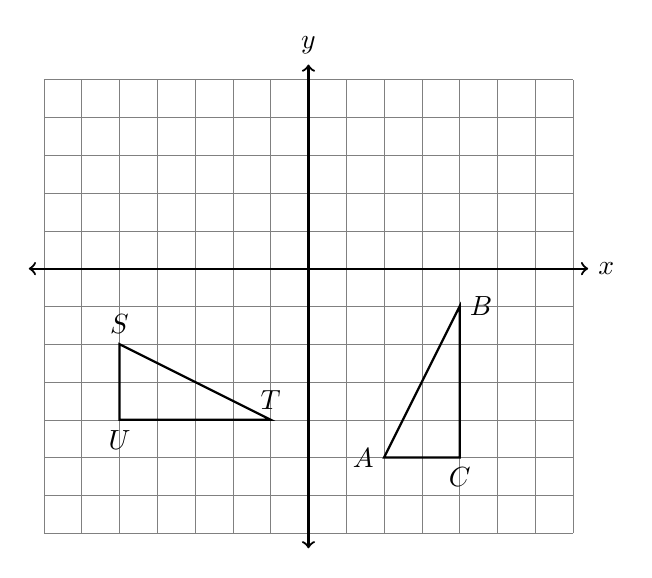
\begin{tikzpicture}[scale=.48]
      \draw [help lines] (-7,-7) grid (7,5);
      \draw [thick, <->] (-7.4,0) -- (7.4,0) node [right] {$x$};
      \draw [thick, <->] (0,-7.4)--(0,5.4) node [above] {$y$};  
      \draw [thick]
        (2,-5) node[left] {$A$}--
        (4,-1) node[right] {$B$}--
        (4,-5) node[below] {$C$}--cycle;
      \draw [thick]
      (-5,-2) node[above] {$S$}--
      (-1,-4) node[above] {$T$}--
      (-5,-4) node[below] {$U$}--cycle;
    \end{tikzpicture}
  \end{flushright}

  \item Rotate $\triangle JKL$ $90^\circ$ clockwise around the origin on the axes below, labeling the image $\triangle J'K'L'$.
  \begin{center}
      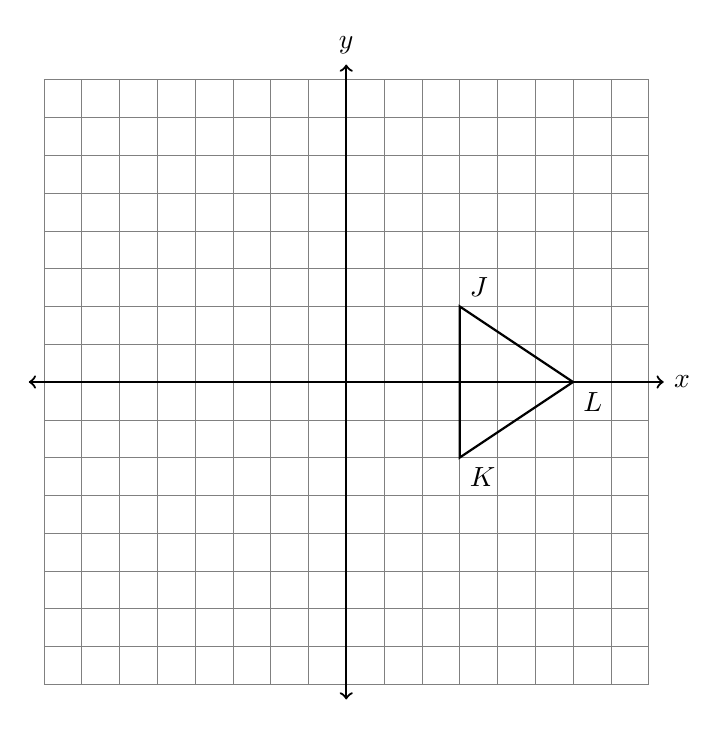
\begin{tikzpicture}[scale=.48]
      \draw [help lines] (-8,-8) grid (8,8);
      \draw [thick, <->] (-8.4,0) -- (8.4,0) node [right] {$x$};
      \draw [thick, <->] (0,-8.4)--(0,8.4) node [above] {$y$};  
      \draw [thick]
        (3,2) node[above right] {$J$}--
        (3,-2) node[below right] {$K$}--
        (6,0) node[below right] {$L$}--cycle;  
    \end{tikzpicture}
  \end{center}

  \newpage
  \item Determine and state the transformation mapping $\triangle BOW$ onto $\triangle TIE$. 
    \begin{flushright}
        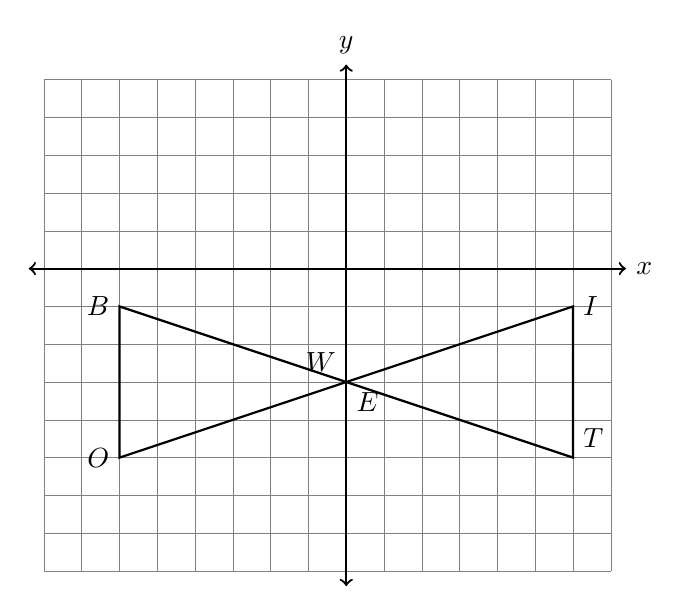
\begin{tikzpicture}[scale=.48]
        \draw [help lines] (-8,-8) grid (7,5);
        \draw [thick, <->] (-8.4,0) -- (7.4,0) node [right] {$x$};
        \draw [thick, <->] (0,-8.4)--(0,5.4) node [above] {$y$};  
        \draw [thick]
          (-6,-1) node[left] {$B$}--
          (-6,-5) node[left] {$O$}--
          (0,-3) node[above left] {$W$}--cycle;
        \draw [thick]
        (6,-1) node[right] {$I$}--
        (6,-5) node[above right] {$T$}--
        (0,-3) node[below right] {$E$}--cycle;
      \end{tikzpicture}
    \end{flushright}

  \item Describe a rigid motion that maps $\triangle TIC$ onto $\triangle TOK$. 
    \begin{flushright}
        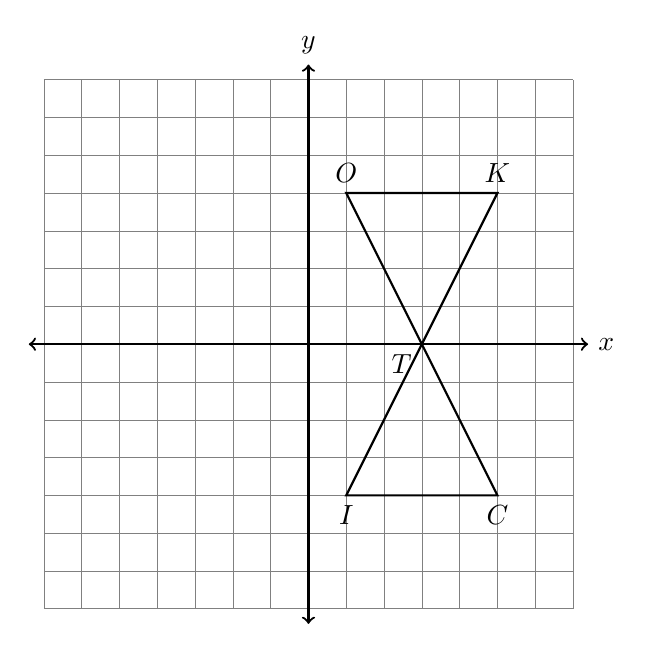
\begin{tikzpicture}[scale=.48]
        \draw [help lines] (-7,-7) grid (7,7);
        \draw [thick, <->] (-7.4,0) -- (7.4,0) node [right] {$x$};
        \draw [thick, <->] (0,-7.4)--(0,7.4) node [above] {$y$};  
        \draw [thick]
          (1,4) node[above] {$O$}--
          (5,4) node[above] {$K$}--
          (3,0) --cycle;
        \draw [thick]
        (1,-4) node[below] {$I$}--
        (5,-4) node[below] {$C$}--
        (3,0) node[below left] {$T$}--cycle;
      \end{tikzpicture}
    \end{flushright}

    \item Find the coordinates of the image of the point $D(3,5)$ after a reflection across the $x$-axis.
    
\newpage    
  \begin{multicols}{2}
    [\item The quadrilateral $MATH$ is mapped to $M'A'T'H'$ by a rigid motion. What transformation a been applied?]  \vspace{0.5cm}
    \begin{enumerate}
      \item Dilation
      \item Reflection
      \item Rotation
      \item Translation
    \end{enumerate}
    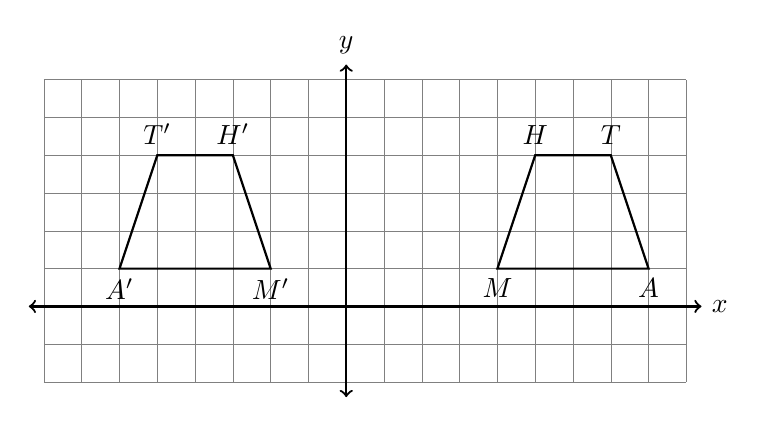
\begin{tikzpicture}[scale=.48]
      \draw [help lines] (-8,-2) grid (9,6);
      \draw [thick, <->] (-8.4,0) -- (9.4,0) node [right] {$x$};
      \draw [thick, <->] (0,-2.4)--(0,6.4) node [above] {$y$};  
      \draw [thick]
        (4,1) node[below] {$M$}--
        (8,1) node[below] {$A$}--
        (7,4) node[above] {$T$}--
        (5,4) node[above] {$H$}--cycle;
      \draw [thick]
        (-2,1) node[below] {$M'$}--
        (-6,1) node[below] {$A'$}--
        (-5,4) node[above] {$T'$}--
        (-3,4) node[above] {$H'$}--cycle; 
    \end{tikzpicture}
  \end{multicols}

  \item Determine and state the sequence of transfromations applied to map $BECA$ to $B''E''C''A''$.
  \begin{flushright}
      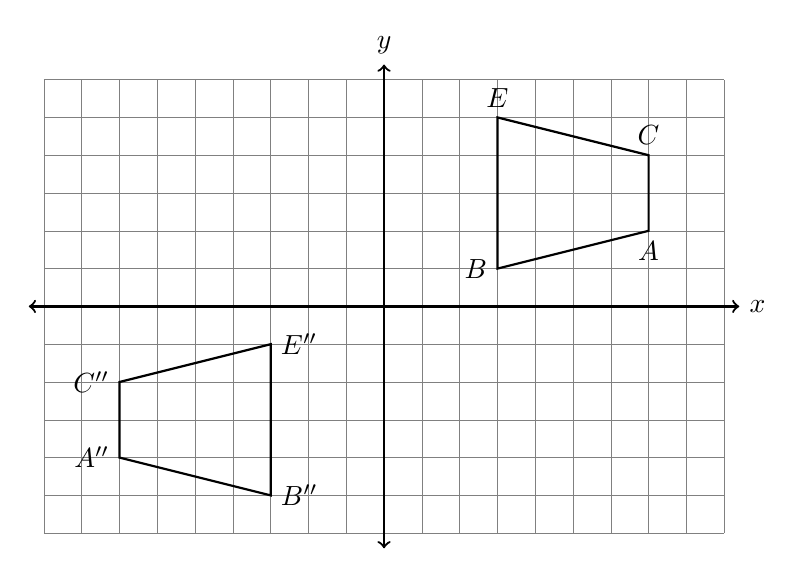
\begin{tikzpicture}[scale=.48]
      \draw [help lines] (-9,-6) grid (9,6);
      \draw [thick, <->] (-9.4,0) -- (9.4,0) node [right] {$x$};
      \draw [thick, <->] (0,-6.4)--(0,6.4) node [above] {$y$};  
      \draw [thick]
        (3,1) node[left] {$B$}--
        (3,5) node[above] {$E$}--
        (7,4) node[above] {$C$}--
        (7,2) node[below] {$A$}--cycle;
      \draw [thick]
        (-3,-1) node[right] {$E''$}--
        (-3,-5) node[right] {$B''$}--
        (-7,-4) node[left] {$A''$}--
        (-7,-2) node[left] {$C''$}--cycle; 
    \end{tikzpicture}
  \end{flushright}
 
  \begin{multicols}{2}
    [\item Which of the following would map $\triangle DOG \rightarrow \triangle D'O'G'$?]  \vspace{0.5cm}
    \begin{itemize}
      \item[T \quad F \quad] $(x,y) \rightarrow (x-6, y+0)$
      \item[T \quad F \quad] Rotated $90^\circ$ clockwise around $(2,0)$      \item[T \quad F \quad] Reflected across the $y$-axis
      \item[T \quad F \quad] Translated six to the left, down zero
      \item[T \quad F \quad] Slid to the left four, then reflected across the $y$-axis
      \item[T \quad F \quad] Reflected across the line $x=2$
    \end{itemize}
    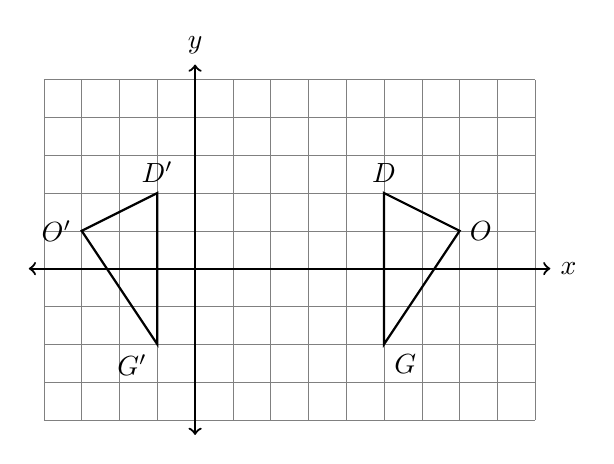
\begin{tikzpicture}[scale=.48]
      \draw [help lines] (-7,-4) grid (6,5);
      \draw [thick, <->] (-7.4,0) -- (6.4,0) node [right] {$x$};
      \draw [thick, <->] (-3,-4.4)--(-3,5.4) node [above] {$y$};  
      \draw [thick]
      (2,2) node[above] {$D$}--
      (4,1) node[right] {$O$}--
      (2,-2) node[below right] {$G$}--cycle;
      \draw [thick]
      (-4,2) node[above] {$D'$}--
      (-6,1) node[left] {$O'$}--
      (-4,-2) node[below left] {$G'$}--cycle;
    \end{tikzpicture}
  \end{multicols}

\newpage

  \item The quadrilateral $KITE$ undergoes rigid motions, shown below. Describe the sequence of transformations applied.
  \begin{flushright}
    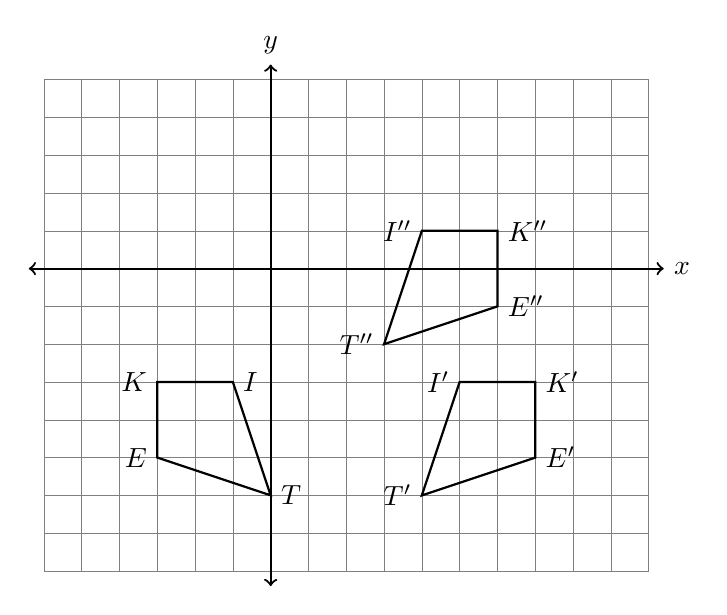
\begin{tikzpicture}[scale=.48]
    \draw [help lines] (-6,-8) grid (10,5);
    \draw [thick, <->] (-6.4,0) -- (10.4,0) node [right] {$x$};
    \draw [thick, <->] (0,-8.4)--(0,5.4) node [above] {$y$};  
    \draw [thick]
    (6,1) node[right] {$K''$}--
    (6,-1) node[right] {$E''$}--
    (3,-2) node[left] {$T''$}--
    (4,1) node[left] {$I''$}--cycle; 
    \draw [thick]
      (7,-3) node[right] {$K'$}--
      (7,-5) node[right] {$E'$}--
      (4,-6) node[left] {$T'$}--
      (5,-3) node[left] {$I'$}--cycle;  
    \draw [thick]
    (-3,-3) node[left] {$K$}--
    (-3,-5) node[left] {$E$}--
    (0,-6) node[right] {$T$}--
    (-1,-3) node[right] {$I$}--cycle;
  \end{tikzpicture}
\end{flushright}

  \item Reflect the rhombus $BECA$ across the $x$-axis, then translated $(x,y) \rightarrow (x+4,y+2)$. Label the images $B'E'C'A'$ and $B''E''C''A''$.
    \begin{center}
        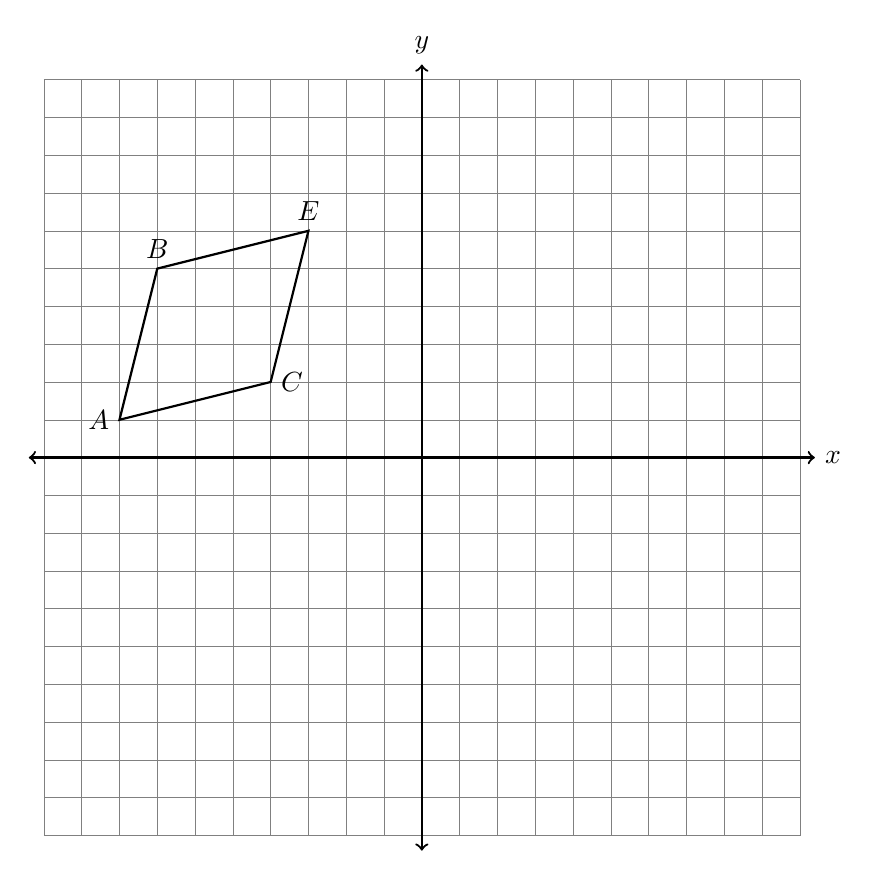
\begin{tikzpicture}[scale=.48]
        \draw [help lines] (-10,-10) grid (10,10);
        \draw [thick, <->] (-10.4,0) -- (10.4,0) node [right] {$x$};
        \draw [thick, <->] (0,-10.4)--(0,10.4) node [above] {$y$};  
        \draw [thick]
          (-4,2) node[right] {$C$}--
          (-3,6) node[above] {$E$}--
          (-7,5) node[above] {$B$}--
          (-8,1) node[left] {$A$}--cycle;  
      \end{tikzpicture}
    \end{center}

\newpage

\begin{multicols}{2}[\item Two triangles are shown with $P$ the intersection of $\overline{AJ}$ and $\overline{BK}$.]
  \begin{enumerate}
    \item Justify $\angle APB \cong \angle JPK$.
    \item What angle must be congruent to $\angle K$ to prove $\triangle ABP \sim \triangle JKP$ by \emph{angle-angle similarity}? \vspace{2cm}
    \end{enumerate}
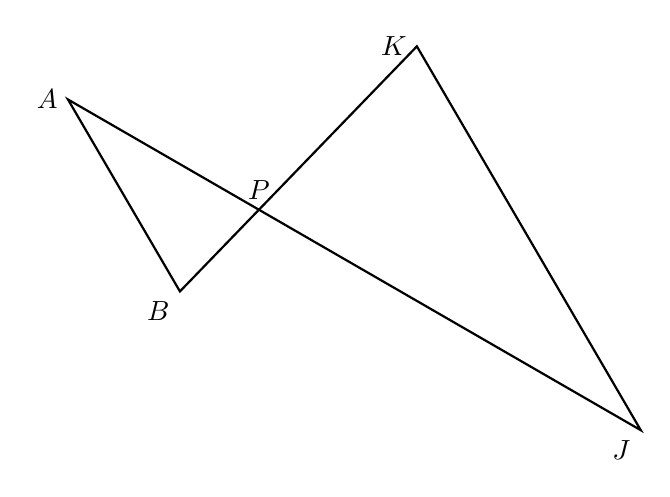
\begin{tikzpicture}[rotate=-30, scale=1.4]
    \draw [thick]
      (-0.25,-1)node[below left]{$B$}--
      (0.5,2)node[left]{$K$}--
      (4,0)node[below left]{$J$}--
      (0,0)node[above]{$P$}--
      (-2,0)node[left]{$A$}--cycle;
  \end{tikzpicture}
\end{multicols}
  \vspace{1cm}

\item Given $\triangle PQR \sim \triangle STU$, $m\angle P=37^\circ$, and $m\angle T=46^\circ$. Find $m\angle R$. \vspace{3cm}

\begin{multicols}{2}[\item The diagram below shows $\triangle ABC$, with $\overline{AEB}$ and $\overline{ADC}$.]
\begin{enumerate}
  \item Justify $\angle BAC \cong \angle DAE$.
  \item What angle must be congruent to $\angle ABC$ to prove $\triangle ABC \sim \triangle ADE$ by \emph{angle-angle similarity}? \vspace{3cm}
\end{enumerate}
  \begin{tikzpicture}[scale=1.3]
    \draw [thick]
    (0,0) node[above right] {$A$}--
    (230:6) node[below left] {$B$}--
    (260:4.75) node[below right] {$C$}--cycle;
    \draw [thick]
    (230:2.375) node[above left] {$E$}--
    (260:3) node[right] {$D$}--cycle;
  \end{tikzpicture}
\end{multicols}

\newpage
\item A dilation centered at the origin with scale factor $k=\frac{1}{2}$ maps $\overline{AB} \rightarrow \overline{A'B'}$. 
\begin{multicols}{2}
\begin{enumerate}
  \item Draw and label the image.
  \item What is the ratio of the length of $\overline{A'B'}$ to $\overline{AB}$?
  \item What is the relationship of the slope of $\overline{A'B'}$ and $\overline{AB}$?
  \begin{flushright}
    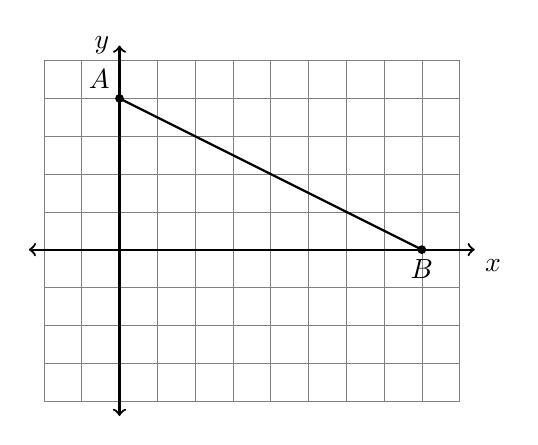
\begin{tikzpicture}[scale=.48]
      \draw [help lines] (-2,-4) grid (9,5);
      \draw [thick, <->] (-2.4,0) -- (9.4,0) node [below right] {$x$};
      \draw [thick, <->] (0,-4.4)--(0,5.4) node [left] {$y$};
      \draw [thick] (0,4)--(8,0);
      \draw [fill] (0,4) circle [radius=0.1] node[above left] {$A$};
      \draw [fill] (8,0) circle [radius=0.1] node[below] {$B$};
    \end{tikzpicture}
  \end{flushright}
\end{enumerate}
\end{multicols} \vspace{1cm}

\item Given $\triangle ABC$, $D$ is the midpoint of $\overline{BA}$, $E$ is a point on $\overline{BC}$, and $\overline{DE}$ is drawn. \\*[2pt] 
If $BA=8$ and $BE=6$, what is the length of $\overline{BC}$ so that $\overline{AC} \parallel \overline{DE}$?
\begin{flushright}
    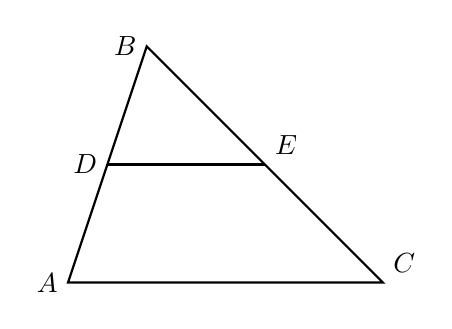
\begin{tikzpicture}[scale=0.5]
      \draw [thick]
      (0,0)node[left]{$A$}--
      (8,0)node[above right]{$C$}--
      (2,6)node[left]{$B$}--cycle;
      \draw [thick]
      (1,3)node[left]{$D$}--
      (5,3)node[above right]{$E$};
    \end{tikzpicture}
  \end{flushright}


\item In diagram below, each centimeter represents six inches. Find the value of each item below in feet.
\begin{multicols}{2}
  \begin{enumerate}[itemsep=1.5cm]
    \item $AC=$
    \item $BC=$
    \item Find the perimeter of $\triangle ABC$
    \item Find the area of $\triangle ABC$
  \end{enumerate}
\begin{center}
  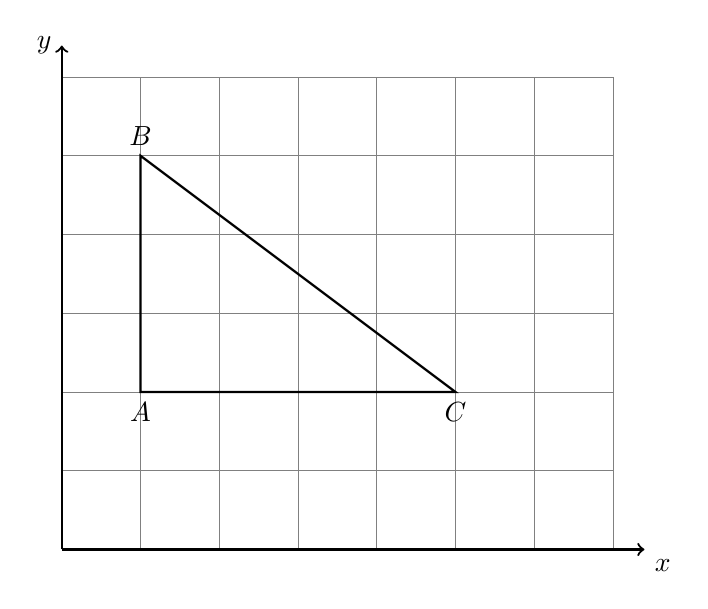
\begin{tikzpicture}
    \draw [help lines] (0,0) grid (7,6);
    \draw [thick, ->] (0,0) -- (7.4,0) node [below right] {$x$};
    \draw [thick, ->] (0,0)--(0,6.4) node [left] {$y$};
    \draw [thick] (1,2)node[below]{$A$}--(5,2)node[below]{$C$}
    --(1,5)node[above]{$B$}--cycle;
  \end{tikzpicture}
\end{center}
\end{multicols}%\vspace{2cm}


\newpage
\item Given $\triangle ABP \sim \triangle JKP$ as shown below. $AB=9.0$, $AP=10.0$, $BP=5.5$, and $AJ=25.0$. Find $JK$.
\begin{flushright}
\begin{tikzpicture}[scale=1.4]
    \draw [thick]
      (-0.25,-1)node[below left]{$B$}--
      (0.5,2)node[left]{$K$}--
      (4,0)node[below left]{$J$}--
      (0,0)node[above left]{$P$}--
      (-2,0)node[left]{$A$}--cycle;
  \end{tikzpicture}
  \end{flushright}
  \vspace{0.5cm}

\item The vertices of $\triangle JKL$ have coordinates $J(-4,-2)$, $K(3,3)$, and $L(-3,5)$, as shown. \\[0.25cm]
Apply a dilation to $\triangle JKL \rightarrow \triangle J'K'L'$, centered at $P(-1,3)$ and with a scale factor $k=2$. Draw the image $\triangle J'K'L'$ on the set of axes below, labeling the vertices.
  \begin{center}
    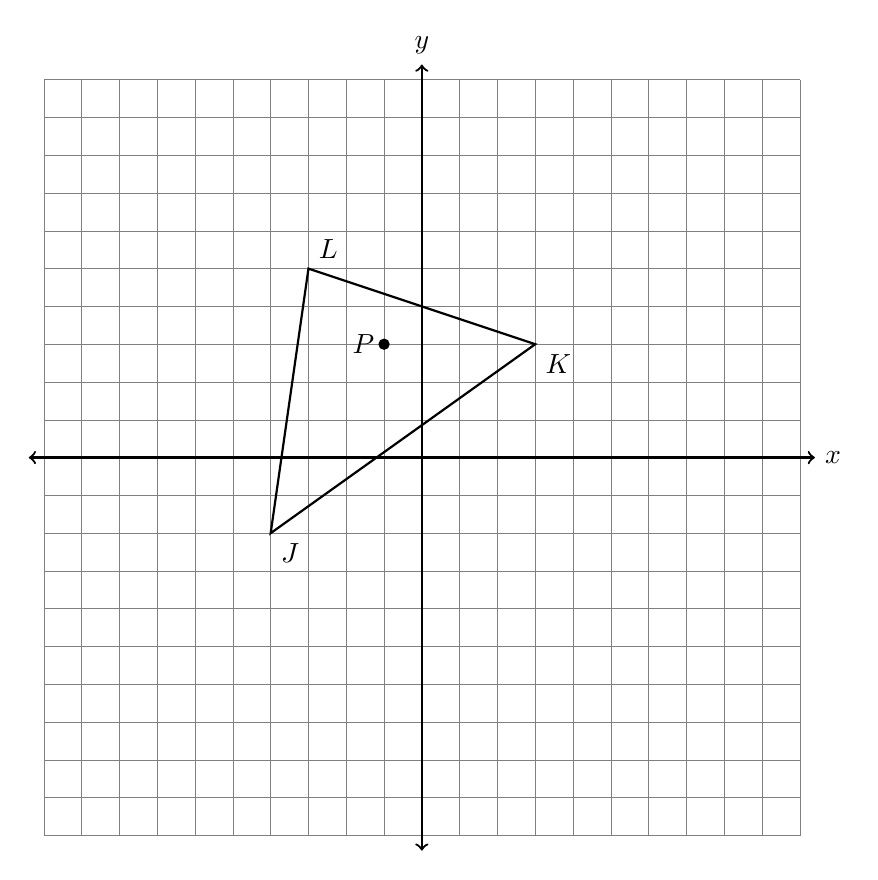
\begin{tikzpicture}[scale=.48]
      \draw [help lines] (-10,-10) grid (10,10);
      \draw [thick, <->] (-10.4,0) -- (10.4,0) node [right] {$x$};
      \draw [thick, <->] (0,-10.4)--(0,10.4) node [above] {$y$};
      \draw [thick]
        (-4,-2) node[below right] {$J$}--
        (3,3) node[below right] {$K$}--
        (-3,5) node[above right] {$L$}--
        cycle;
      \fill (-1,3) circle[radius=0.15cm]node[left]{$P$};
    \end{tikzpicture}
  \end{center}
  What is the ratio of the area of $\triangle JKL$ to $\triangle J'K'L'$?

\newpage
\item In $\triangle ABC$ shown below, $\angle ACB$ is a right angle, $E$ is a point on $\overline{AC}$, and $\overline{ED}$ is drawn perpendicular to hypontenuse $\overline{AB}$.
\begin{center}
  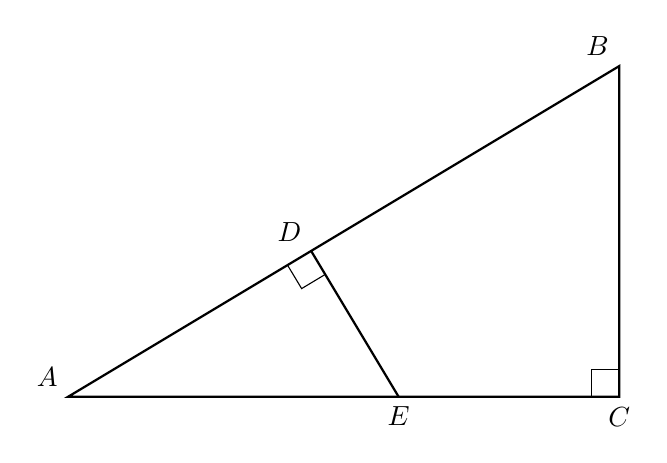
\begin{tikzpicture}[scale=0.7]
    \draw [-, thick] (0,0) node[above left]{$A$}--
    (10,0) node[below]{$C$}--
    (10,6) node[above left]{$B$}--cycle;
    \draw [thick] (6,0)--(4.41,2.65);
    \node at (6,0) [below]{$E$};
    \node at (4.41,2.65) [above left]{$D$};
    \draw (10,0) ++(-0.5,0)--++(0,0.5)--++(0.5,0);
    \draw (4.41,2.65) ++(-59:0.5)--++(-149:0.5)--++(121:0.5);
    %\node at (4, 0) [below]{$12$};
    %\node at (3,2) [above]{$9$};
    %\node at (9, 3) [right]{$10$};
    %\node at (5.5, 1.6) [right]{$6$}; \vspace{1cm}
  \end{tikzpicture}
\end{center} 
If $AB = 9$, $BC = 6$, and $DE = 4$, what is the length of $\overline{AE}$? \vspace{3cm}

\item In the diagram below, $\angle ABC \cong \angle ADE$, $AB = 9$, $AC = 6$, $BD = 13.5$, and $DE = 16$. Find  $AD$ and the scale factor $k$. Then find $AE$ and $BC$. %\vspace{1cm}
\begin{multicols}{2}
\begin{enumerate}
  \item $AD=$ \vspace{0.3cm}
  \item $k=$ \vspace{0.3cm}
  \item $AE=$ \vspace{0.3cm}
  \item $BC=$
\end{enumerate}
\begin{flushright}
  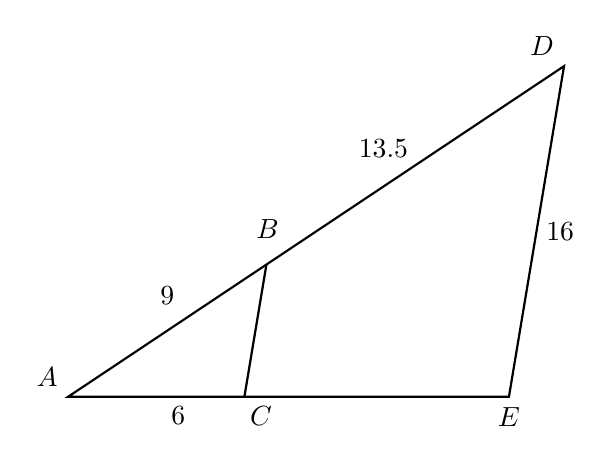
\begin{tikzpicture}[scale=0.7]
    \draw [-, thick] (0,0) node[above left]{$A$}--
    (8,0) node[below]{$E$}--
    (9,6) node[above left]{$D$}--cycle;
    \draw [thick] (3.2,0)--(3.6,2.4);
    \node at (3.5,0) [below]{$C$};
    \node at (4,2.7) [above left]{$B$};
    \node at (2, 0) [below]{$6$};
    \node at (1.8,1.5) [above]{$9$};
    \node at (8.5, 3) [right]{$16$};
    \node at (5.1, 4.5) [right]{$13.5$}; \vspace{1cm}
  \end{tikzpicture}
\end{flushright} 
\end{multicols}\vspace{1cm}

\newpage
\item The line $\overleftrightarrow{AB}$ has the equation $y=\frac{2}{3}x-2$. Apply a dilation mapping $\overleftrightarrow{AB} \rightarrow \overleftrightarrow{A'B'}$ with a factor of $k=3$ centered at the origin. Draw and label the image on the grid. Write the equation of the line $\overleftrightarrow{A'B'}$.
\begin{flushright} %4 quadrant regents grid w T-Chart
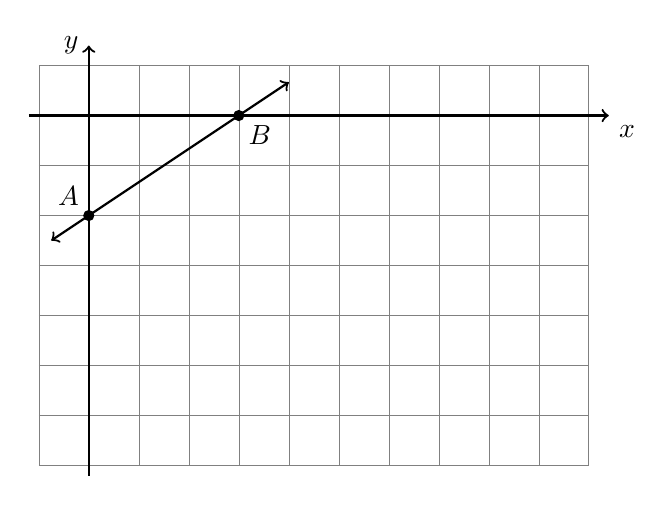
\begin{tikzpicture}[scale=.635]
  \draw [help lines] (-1,-7) grid (10,1);
  \draw [thick, ->] (-1.2,0) -- (10.4,0) node [below right] {$x$};
  \draw [thick, ->] (0,-7.2)--(0,1.4) node [left] {$y$};
  \draw [<->, thick] (-0.75,-2.5)--(4,0.667);
  \draw [fill] (0,-2) circle [radius=0.1]node[above left]{$A$};
  %\draw [fill] (3,0) circle [radius=0.1]node[below left]{$C$};
  \draw [fill] (3,0) circle [radius=0.1]node[below right]{$B$};
\end{tikzpicture}
\end{flushright}

\begin{multicols}{2}[\item The diagram below shows $\triangle ABC$. $E$ bisects $\overline{AB}$, and $\angle ACB \cong \angle AED$. $AB=18$, $AC=12$, and $DE=7$. Find the scale factor $k$, $BC$, and $AD$.]
\begin{enumerate}
  \item $k=$ \vspace{1cm}
  \item $BC=$ \vspace{1cm}
  \item $AD=$  \vspace{1cm}
\end{enumerate}
  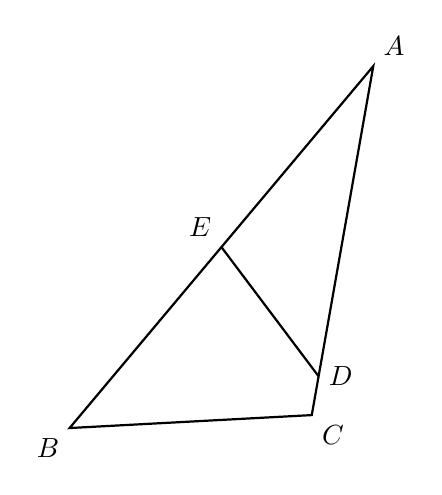
\begin{tikzpicture}[scale=1.0]
    \draw [thick]
    (0,0) node[above right] {$A$}--
    (230:6) node[below left] {$B$}--
    (260:4.5) node[below right] {$C$}--cycle;
    \draw [thick]
    (230:3) node[above left] {$E$}--
    (260:4) node[right] {$D$}--cycle;
  \end{tikzpicture}
\end{multicols}\vspace{0.5cm}

\item In the diagram below, the chords $\overline{AE}$ and $\overline{BD}$ intersect at $C$. Given $\triangle ABC \sim \triangle DEC$, $BC=6$, $CD=12$, and $CE=10$. Determine the length of $\overline{CA}$.
\begin{flushright}
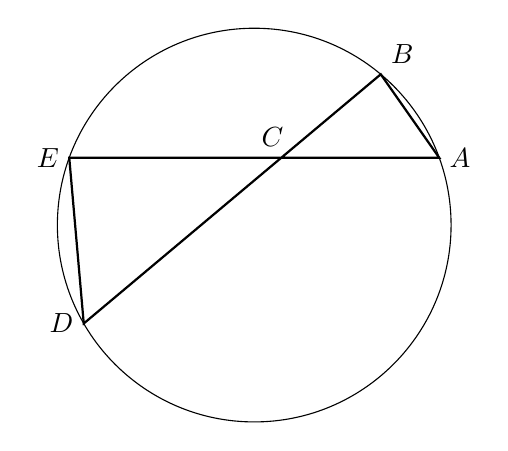
\begin{tikzpicture}[scale=.5]
  \draw (0,0) circle[radius=5];
  \draw [thick]
  (20:5) node[right] {$A$}--
  (160:5) node[left] {$E$}--
  (210:5) node[left] {$D$}--
  (50:5) node[above right] {$B$}--cycle;
  \draw (75:1.8) node[above] {$C$};
\end{tikzpicture}
\end{flushright}

\newpage
\item Determine and state the sequence of transformations applied to map $\triangle ABC \rightarrow \triangle DEF$.
\begin{flushright}
    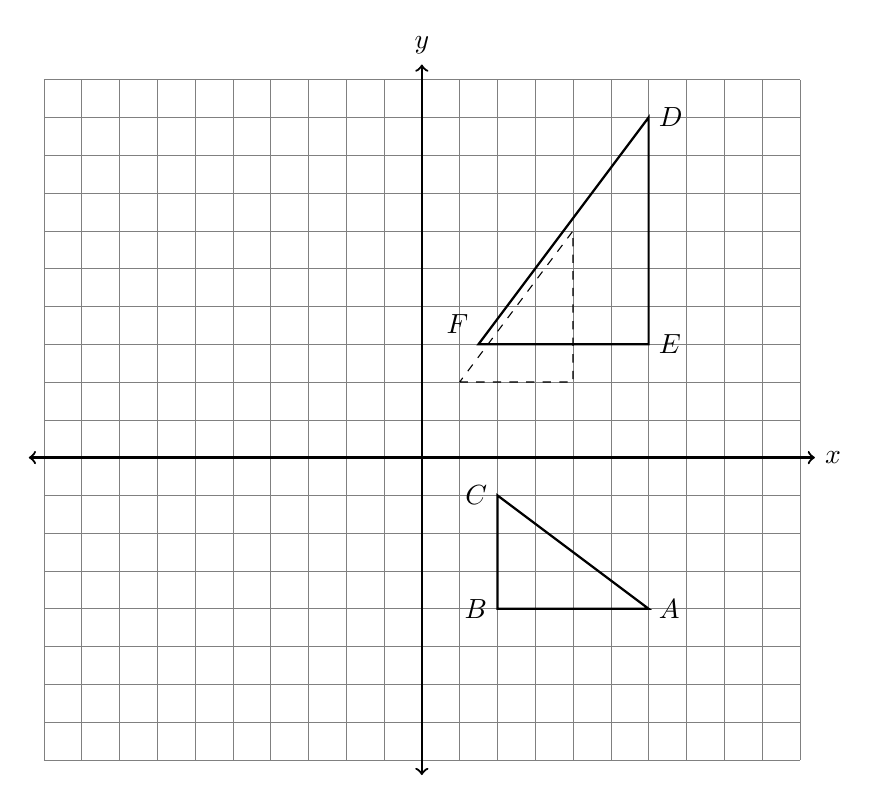
\begin{tikzpicture}[scale=.48]
    \draw [help lines] (-10,-8) grid (10,10);
    \draw [thick, <->] (-10.4,0) -- (10.4,0) node [right] {$x$};
    \draw [thick, <->] (0,-8.4)--(0,10.4) node [above] {$y$};  
    \draw [thick]
    (1.5,3) node[above left] {$F$}--
    (6,3) node[right] {$E$}--
    (6,9) node[right] {$D$}--cycle;
    \draw [thick]
      (2,-1) node[left] {$C$}--
      (2,-4) node[left] {$B$}--
      (6,-4) node[right] {$A$}--cycle; 
      \draw [dashed]
    (1,2) --
    (4,2) --
    (4,6) --cycle;
  \end{tikzpicture}
\end{flushright}

\item What sequence of transformations would map $\triangle ABC$ onto $\triangle DEF$?
\begin{flushright}
    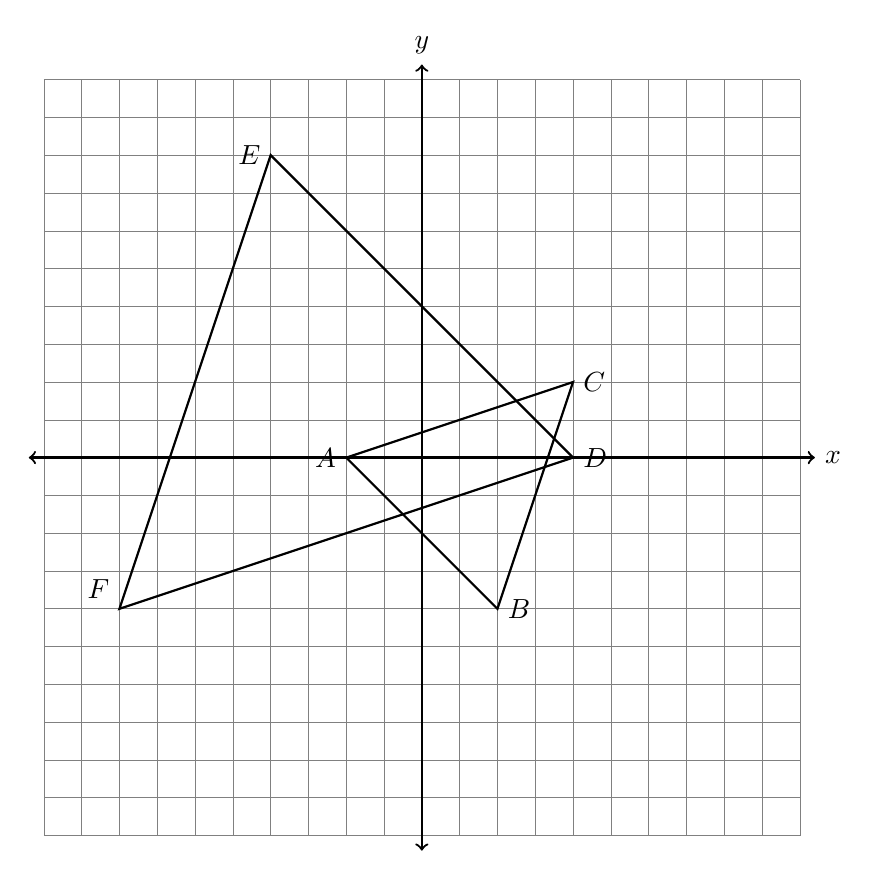
\begin{tikzpicture}[scale=.48]
    \draw [help lines] (-10,-10) grid (10,10);
    \draw [thick, <->] (-10.4,0) -- (10.4,0) node [right] {$x$};
    \draw [thick, <->] (0,-10.4)--(0,10.4) node [above] {$y$};  
    \draw [thick]
    (-8,-4) node[above left] {$F$}--
    (-4,8) node[left] {$E$}--
    (4,0) node[right] {$D$}--cycle;
    \draw [thick]
      (4,2) node[right] {$C$}--
      (2,-4) node[right] {$B$}--
      (-2,0) node[left] {$A$}--cycle; 
  \end{tikzpicture}
\end{flushright}

  
\end{enumerate}
\end{document}

